\documentclass[11pt, notitlepage]{report}

\usepackage[margin=0.75in]{geometry}
\usepackage{amssymb}
\usepackage{amsmath}
\usepackage{tensor}

\usepackage{setspace}
\usepackage{braket}
\usepackage{tikz-feynman}
\usetikzlibrary{patterns, decorations.markings, positioning}

\usepackage{xcolor}
\usepackage[colorlinks=true, urlcolor=blue, linkcolor=blue]{hyperref}

\usepackage{tocloft}
\renewcommand{\cftsecleader}{\cftdotfill{\cftdotsep}} % for sections, if you really want! (It is default in report and book class (So you may not need it).

\renewcommand{\thesection}{\arabic{section}}

\setstretch{1.3}

\newcommand{\bul}{\(\bullet\)}
\newcommand{\del}{\partial}
\newcommand{\z}{\mathcal{Z}}
\newcommand{\real}{\mathbb{R}}
\newcommand{\complex}{\mathbb{C}}
\newcommand{\e}{\mathrm{e}}
\newcommand{\w}{\omega}
\newcommand{\D}{\mathcal{D}}
\newcommand{\ld}{\mathcal{L}}
\newcommand{\hd}{\mathcal{H}}
\newcommand{\normord}[1]{:\mathrel{#1}:}
\renewcommand{\a}[1]{a_\mathbf{#1}}
\newcommand{\adag}[1]{a^\dagger_\mathbf{#1}}

\numberwithin{equation}{section}


\setlength{\parindent}{0pt}

\title{Quantum Field Theory I}
\author{Instructor: Dr.\ Suvrat Raju\vspace{30pt}\\ Adithya A. Rao}
\date{~}
\begin{document}
    \maketitle

    \pagenumbering{roman}
    This is the lecture notes for Prof.\ Suvrat Raju's course on Quantum Field Theory I, given at ICTS Bangalore in the semester Jan-April 2024.
    The course is available on youtube \href{https://youtu.be/9kqScPIkkRU?si=UH9KUZaF0YiDwxdu}{here}. \\
    There are a few sections in the notes which are in red. These are statements and calculations that I have done and concluded on my own and are not stated or performed in the lecture.\\
    If you find any errors in the text, please send an email to me at \href{mailto:adithyarao3132001@gmail.com}{adithyarao3132001@gmail.com}

    \thispagestyle{empty}
    \tableofcontents
    \newpage
    \setcounter{page}{1}
    \pagenumbering{arabic}

    \addcontentsline{toc}{chapter}{Introduction — The Machinery of QFT}

    
    \section{The Need for Fields}
    Quantum field theory is your normal quantum mechanics generalised to infinite number of degrees of freedom, where the dynamics of interactions between these infinite degrees of freedom is consistent with the postulates of Special Theory of Relativity (STR).\\

    The question is then why these infinite number of degrees of freedom are needed. In non-relativistc classical mechanics, one sees that there is a requirement of only \(6N\) number of degrees of freedom at-most, when describing the dynamics involving \(N\) particles, but when transitioning to QFT, why does describing even \(2\) particles require inifnite degrees of freedom? 

    \subsection{ANY Dynamics Consistent with STR Demand Infinite Degrees of Freedom}
    Consider two particles, at the same time slice \(t\) in some reference frame at positions \(x_1~\&~x_2\) interacting with each other. Consistency with STR requires that the force on particle 1 due to 2 at this instant should depend on the retarded position of the particle 2 and not the position at that instant. 

    \input{diagrams/worldlines.tex}
    
    \begin{equation}
        F_{12} = F(x_2(t-\tau_2), \dot{x_2}(t-\tau_2), \dots, x_1(t), \dot{x_1}(t), \dots)
    \end{equation}
    and similarly
    \begin{equation}
        F_{21} = F'(x_1(t-\tau_1), \dot{x_1}(t-\tau_1), \dots, x_2(t), \dot{x_2}(t), \dots)
    \end{equation}
    In such an equation, the \(\tau_1\) and \(\tau_2\) themselves are dynamically determined, and depend on the entire past history of the two particles, and therefore in order to determine the dynamics of the particles, one needs to keep track of functions, which have infinite degrees of freedom. \\

    That said, even in classical dynamics, imposing STR postulates demands infinite number of degrees of freedom. 

    \subsection{Quantizing the STR Dynamics}
    In dealing with such systems, we encounter \textit{retarded differential equations}, or also called as \textit{functional differential equations}. And nobody knows how to quantize the system starting from the functional differential equations.\\

    Passage from CM to QM relies strongly on the idea that we are given an initial surface and we have a Hamiltonian/Lagrangian on it.\\
    In a Hamiltonian system we have a phase space and we see how stuff evolves in that space. In the above discussed case, we have to deal with an infinite number of degrees of freedom and these degrees of freedom are not in the form that is convenient to put in the Hamiltonian formalism.\\

    Fields solve this problem by rather than saying that particle 1 interacts with particle 2, we say particle 1 interacts with a field, and particle 2 too interacts with the field. The field and the particles influence each other only locally. In introducing this formalism we paid a price, we introduced infinite number of degrees of freedom in the form of fields, at the effect of removing the necessity of having to track all particle histories. The field can be thought of as keeping track of the history of the particles. In the language of fields, nothing depends on retarded times. \\

    With the introduction of fields, we now have everything in the language of phase space. We are given an initial surface, and data on it, and we can evolve everything into future. But rather than having only finite degrees of freedom we still need to keep track of infinite degrees of freedom of the fields, but they are now in a form convenient to quantize.\\

    \subsection{Another Reason Why We Need Infinite DOFs}
    Heisenberg's uncertainity principle — \(\Delta x \Delta p \ge1 \)\\
    If we have small \(\Delta x\), then \(\Delta p \) becomes large, such that \(\Delta E \ge m\). In this case we are now uncertain if we are dealing with the original particle, or if we have created a new particle. It is convenient therefore, to discuss the particles as excitations of fields, using which one can describe variable number of particles.\\

    ALSO fields explain why all electrons are identical.\\

    \subsection{Regular QM Breaks Causality}
    This is a very generic calculation that can be found in almost all lectures/texbooks. But still included here for completeness. \\

    The regular, single particle quantum mechanics that we all know of and are familiar with breaks causality. Causality requires that a particle can never move faster than the speed of light, i.e.\ a particle initially localised around the position \(\textbf{x}\) should not have any amplitude to move out of the future light cone. Now in the case of single particle QM, consider a particle localised about \(\textbf{x}\), described by state \(\ket{\textbf{x}}\).\\

    Suppose the particle follows the relativistic Hamiltonian, \(\hat H = \sqrt{\hat{\textbf{p}}^2 + m^2}\), the state of the particle after time \(t\) would be \(\exp(-i H t) \ket{\textbf{x}}\). Relativity requires that this state should have zero overlap with \(\ket{\textbf{x}'}\) where \((t, \textbf{x})\) and \((t, \textbf{x}')\) are spacelike separated.\\

    Let \(G(\textbf{x},\textbf{x}') = \braket{\textbf{x}' | \exp(-iHt) \textbf{x}}\). The explicit value of \(G\) can be calculated by inserting the identity in \(\ket{\textbf{p}}\) as follows.

    \begin{equation}
        G(\textbf{x}, \textbf{x}', t) = \int \frac{d^3\textbf{p}}{(2\pi)^3} \braket{\textbf{x}' | \exp(-i\sqrt{\hat{\textbf{p}}^2 + m^2} t) | \textbf{p}} \braket{\textbf{p}|\textbf{x}} = \int \frac{d^3\textbf{p}}{(2\pi)^3} \exp(-i\sqrt{\textbf{p}^2 + m^2} t)\braket{\textbf{x}'| \textbf{p}} \braket{\textbf{p}|\textbf{x}}
    \end{equation}
    \begin{equation}
        G(\textbf{x},\textbf{x}', t) = \int \frac{d^3\textbf{p}}{(2\pi)^3}  \exp(-i\sqrt{\textbf{p}^2 + m^2} t) \exp(-i \textbf{p}\cdot(\textbf{x}-\textbf{x}'))
    \end{equation}
    Write \(\textbf{x} - \textbf{x}' = \textbf{r}\), and align the \(z\) axis to be about \(\textbf{r}\). Then we can convert the above integral into polar coordinates as (where we use \(p = |\textbf{p}|\) and \(r = |\textbf{r}|\))
    \begin{align}
        G(\textbf{r}, t) &= \int \frac{p^2}{(2\pi)^2} \exp(-i\sqrt{p^2 + m^2} t) \exp(-i p r \cos\theta)~ dp d(\cos\theta)\\
        &= \int \frac{p^2}{(2\pi)^2} \exp(-i\sqrt{p^2 + m^2} t) \left( \frac{\exp(-ipr) - \exp(ipr)}{pr} \right)dp\\
        &= \frac{2}{(2\pi)^2}\frac{1}{r}\int \exp(-i\sqrt{p^2 + m^2} t)~ p ~\sin(pr)~dp
    \end{align}
    You can look up this integral in some Russian textbook and find out that this is equal to 
    \begin{equation}
        G \propto K_2 (m\sqrt{r^2 + t^2}) 
    \end{equation}
    This is some finite non-zero number (although it might be small for some values) for all \(r\) and \(t\). Since we require causality to be exactly held, and not approximately held, single particle quantum mechanics breaks causality.

    \newpage
    \section{Classical Field Theory}
    Everything we discussed previously does not logically conclude that the \textit{only} candidates are fields, but fields provide a convenient formalism, and end up solving the problems we were facing. \\

    In general, field is something associated with spacetime. That is, for every spacetime point, it spits out some mathematical entity. For the field, we would like to write a Lagrangian, as an integral of some Lagrangian density over all space. 
    \begin{equation}
        L = \int\ld ~d^3\textbf{x}
    \end{equation}
    We consider Lagrangian densities of the form 
    \begin{equation}
        \ld(\del_\mu \phi(x), \phi(x))
    \end{equation}
    (where we assume the notation \(x = (t, \textbf{x})\)). In principle, the Lagrangian density can be anything, but mostly we consider the most simple forms. We usually start with something that is quadratic in fields and their derivatives. Linear term is ignored since it can be absorbed into the quadratic term by considering a shift by constant factor of the fields leading to the a quadratic Lagrangian.\\
    Example — suppose
    \begin{equation}
        \ld = \frac{1}{2} (\del_\mu \phi)^2 - \frac{1}{2}m^2 \phi^2 - \alpha \phi
    \end{equation}
    consider the transformation \(\phi(x) \to \phi(x) + \displaystyle\frac{\alpha}{m^2}\), with \(\alpha\) being some spacetime independent constant. 
    \begin{equation}
        \ld' = \frac{1}{2} \left( \del_\mu \left(\phi' - \frac{\alpha}{m^2}\right)\right)^2 - \frac{1}{2} m^2 \left(\phi'^2 - 2\frac{\alpha}{m^2} \phi' + \left(\frac{\alpha}{m^2}\right)^2\right) - \alpha \phi = \frac{1}{2} (\del_\mu \phi')^2 - \frac{1}{2}m^2 \phi'^2
    \end{equation}
    (dynamics doesn't change when a constant term is added to the Lagrangian) which is a Lagrangian density with only quadratic terms. 

    \subsection{Dynamics in Classical Field Theory}
    \subsubsection{Lagrangin Dynamics}
    Action — \(S = \int \ld~d^4x\)
    \begin{center}
        \fbox{Nature is lazy}
    \end{center}
    Classical equations of motion — field configurations such that variation of \(S\) under \(\phi \to \phi + \delta\phi\) is zero. \\
    Under such change, 
    \begin{equation*}
        \delta S = \int \frac{\delta \ld}{\delta \del_\mu \phi}\delta(\del_\mu \phi) + \frac{\delta \ld}{\delta \phi}\delta(\phi) ~d^4x
    \end{equation*}
    \begin{equation}
        = \int -\delta\phi \del_\mu\frac{\delta \ld}{\delta \del_\mu \phi} + \delta\phi\frac{\delta \ld}{\delta \phi} + \del_\mu \left( \delta\phi \frac{\delta \ld}{\delta \del_\mu \phi} \right)~d^4x  
    \end{equation}
    Considering variations which vanish at infinity, the last term (which is only a boundary term) vanishes. The other two functions also should vanish for every possible values of \(\delta \phi\), therefore we get the equations of motions to be 
    \begin{equation}
        \del_\mu\frac{\delta \ld}{\delta \del_\mu \phi} - \frac{\delta \ld}{\delta \phi} = 0
    \end{equation}

    \subsubsection{Hamiltonian Dynamics}
    In order to make a passage to QFT, we need a Hamiltonian formulation. In going to Hamiltonian formulation, we trade the \textit{time derivative} with the \textit{conjugate momentum}.\\

    The basic degrees of freedom in classical mechanics were the spatial points \(\textbf{x}\). In the case of the field theory, the basic degrees of freedom are just the fields at a certain instant of time (which we conveniently call \(t=0\)) \(\psi(\textbf{x})\). The \(\del_i \phi(\textbf{x})\) are nothing but linear combinations of the \(\phi(\textbf{x})\), and in going to the Hamiltonian formulation, we treat the time derivative as a different degree of freedom.

    \begin{equation}
        \Pi(t=0, \textbf{x}) = \dot{\phi}(t=0, \textbf{x})
    \end{equation}

    The Hamiltonian is then 
    \begin{equation}
        H(t) = \int \Pi \dot{\phi} - \ld ~d^3\textbf{x} = \int \hd~d^3\textbf{x}
    \end{equation}
    and one can write equations similar to the Hamiltonian equations of motion for the field and its conjugate momenta.

    \subsection{Parameterizing the Phase Space}
    Given the phase space, the usual parameterization is using \(\Pi\) and \(\Phi\). But we can also parameterize the phase space using different variables — the set of solutions to the equations of motion. This is true because given a point in phase space, we can use it as initial conditions and obtain a solution to the equations of motion. Therefore, there is a one-to-one map between points in phase space and solutions to the equations of motion, and we can see the set of solutions to the equations of motion as parameterizing the phase space. That is, a point corresponds to a solution, and a solution provided a section corresponds to a point.\\
    In other words, the \textit{parameterization} of all solutions to the equations of motion is the same as parameterization of the whole phase space. \\

    For concreteness, let us start considering a specific theory — the scalar free field theory. 
    \begin{equation}
        \ld = \frac{1}{2}\left((\del_\mu \phi)^2 - m^2\phi^2\right)
    \end{equation}
    The equation of motion arising from this lagrangian is simply 
    \begin{equation}
        (\del_\mu \del^\mu + m^2)\phi(x) = (\del_t^2 - \nabla^2 + m^2)\phi(x) = 0
    \end{equation}
    We want to find all possible solutions to this equations of motion in order to parameterize the phase space. To find a parameterization for the solution of the equations of motion, the easiest way is to go to the fourier space. \\
    Writing \(\phi(t, \textbf{x}) = \int d^3\textbf{p} \phi(t, \textbf{p})\exp(i\textbf{p}\cdot\textbf{x})\), we get 
    \begin{equation}
        \int (\del_t^2 + \textbf{p}^2 + m^2)\phi(t, \textbf{p}) d^3\textbf{p} = 0
    \end{equation}
    We are keeping time as it is because in Hamiltonian formulation we require solutions at a given slice of time. \\
    The solutions to the above equation of motion is (with \(\w_\textbf{p} = \sqrt{\textbf{p}^2 + m^2}\))
    \begin{equation}
        \phi(t,\textbf{p}) = a(\textbf{p})\exp(-i \w_\mathbf{p} t) + b(\textbf{p}) \exp(i \w_\mathbf{p} t)
    \end{equation}
    Since we require \(\phi(t, \textbf{x})^* = \phi(t, \textbf{x})\), we need 
    \(\phi(t, \textbf{p})^* = \phi(t, -\textbf{p})\), meaning
    \begin{equation*}
        a^*(\textbf{p})\exp(i \w_\mathbf{p} t) + b^*(\textbf{p}) \exp(-i \w_\mathbf{p} t) = a(-\textbf{p})\exp(-i \w_\mathbf{p} t) + b(-\textbf{p}) \exp(i \w_\mathbf{p} t)
    \end{equation*}
    Comparing, we get \(b(\textbf{p}) = a^*(-\textbf{p})\), therefore, the solutions are 
    \begin{equation}
        \phi(t, \textbf{p}) = a(\textbf{p}) \exp(-i\w_\textbf{p} t) + a^*(-\textbf{p}) \exp(i\w_\textbf{p} t)
    \end{equation}
    and 
    \begin{equation}
        \phi(t, \textbf{x}) = \int a(\textbf{p}) \exp(-i\w_\textbf{p} t + i\textbf{p}\cdot \textbf{x}) + a^*(\textbf{p}) \exp(i\w_\textbf{p} t - i\textbf{p}\cdot \textbf{x}) ~ \frac{1}{\sqrt{2\w_\textbf{p}}} \frac{d^3 \textbf{p}}{(2\pi)^3} 
    \end{equation}
    where in second term, we did the change \(\textbf{p}\to -\textbf{p}\) since the integral is invarient under this change, and \(\displaystyle\frac{1}{\sqrt{2\w_\textbf{p}}}\) is simply a choice of normalisation.\\

    We can also write this as 
    \begin{equation}
        \phi(x) = \int a(p) \exp(-ip.x) + a^*(p) \exp(ip.x) ~\frac{1}{\sqrt{2\w_\textbf{p}}} \frac{d^3 \textbf{p}}{(2\pi)^3} 
    \end{equation}
    where now \(p\) and \(x\) are 4-vectors.\\

    The coordinates on the phase space are \(\phi(t=0, \textbf{x})\) and \(\Pi(t=0, \textbf{x})\), and in this case the parameterization is very clear that 
    \begin{equation}
        \phi(t=0, \textbf{x}) = \int a(\textbf{p}) \exp(i\textbf{p}\cdot \textbf{x}) + a^*(\textbf{p}) \exp(- i\textbf{p}\cdot \textbf{x}) ~ \frac{1}{\sqrt{2\w_\textbf{p}}} \frac{d^3 \textbf{p}}{(2\pi)^3}
    \end{equation}
    and 
    \begin{equation}
        \Pi(t=0, \textbf{x}) = \int -i \left(a(\textbf{p}) \exp(i\textbf{p}\cdot \textbf{x}) - a^*(\textbf{p}) \exp(- i\textbf{p}\cdot \textbf{x}) \right)~ \sqrt{\frac{\w_\textbf{p}}{2}} \frac{d^3 \textbf{p}}{(2\pi)^3}
    \end{equation}
    Rather than parameterizing the phase space using the field and conjugate momentum, we can parameterize using the \(a(\textbf{p})\) and \(a^*(\textbf{p})\). We can also invert these relations to write \(a\) and \(a^*\) in terms of field and momenta.
    \begin{equation}
        a(\textbf{p}) = \sqrt{\frac{\w_\textbf{p}}{2}}\int\phi(0, \textbf{x}) \e^{-i \textbf{p}. \textbf{x}}d^3\textbf{x} + \frac{i}{\sqrt{2\w_\textbf{p}}}\int \Pi(0, \textbf{x})\e^{-i \textbf{p}.\textbf{x}} d^3\textbf{x} 
    \end{equation}
    \begin{equation}
        a^*(\textbf{p}) = \sqrt{\frac{\w_\textbf{p}}{2}}\int\phi(0, \textbf{x}) \e^{i \textbf{p}. \textbf{x}}d^3\textbf{x} - \frac{i}{\sqrt{2\w_\textbf{p}}}\int \Pi(0, \textbf{x})\e^{i \textbf{p}.\textbf{x}} d^3\textbf{x} 
    \end{equation}\\

    \textcolor{red}{
        In order to understand this better, let us do the same analysis for the simpler classical mechanical system of a harmonic oscillator. The equation of motion is 
        \begin{equation*}
            ( \del_t^2 + \w^2 )x = 0
        \end{equation*} This is solved simply by 
        \begin{equation*}
            x(t) = \frac{1}{\sqrt{2\w}}\left(A\exp(-i\w t) + A^*\exp(i\w t)\right) ~~~\because~x\text{ is real}
        \end{equation*}
        where the prefactor is simply a choice of normalisation, and 
        \begin{equation*}
            p(t) = -i\sqrt{\frac{\w}{2}} (A\exp(-i\w t) - A^* \exp(i \w t))
        \end{equation*}
        The coordinates on the phase space are \(x(t=0)\) and \(p(t=0)\), which in this case are 
        \begin{equation*}
            x = \frac{1}{\sqrt{2\w}}(A + A^*)~~\&~~p = -i\sqrt{\frac{\w}{2}} (A - A^*)
        \end{equation*}
        For every \(x, p\), there is a solution \(A\) (where \(A\) is complex) that has \((x,p)\) as its initial conditions, and therefore the set of \(A\) can be thought of as parameterizing the entire phase space. This is exactly what is done in introducing the ladder operators for quantizing the harmonic oscillator. Instead of imposing the quantization condition on the usual coordinates \(x\) and \(p\), one uses the coordinates \(A\) and \(A^*\) and quantizes these degrees of freedom. \\
        Important! — There can be confusion in what one calls a solution to the equation of motion. One might be tempted to assume that, for example in this case, the set of ellipses in the phase space to be the set of solutions to the equations of motions. This is wrong, in the sense that the solutions for motion with initial state \(x_1, p_1\) and with initial state \(x_2, p_2\), even if both lie on the same ellipse, are different. Therefore, given an initial point in phase space, we determine a unique equation that governs this initial point's evolution and this equation is termed a solution. Therefore, corresponding to every point on the phase space, there is a unique solution, and therefore a bijection.  \\      
        }

        \textcolor{red}{
            We can further extend the above discussion by looking at the commutator relations of \(A\) and \(A^*\), which is given by 
            \begin{equation*}
                \{x,p\} = 1 \implies \{A^*, A\} = -i, ~\{A, A\}=0,\{A^*, A^*\} = 0 
            \end{equation*}
            We can also construct the Hamiltonian in terms of the variables \(A\) and \(A^*\), which is given as 
        \begin{equation*}
            H = \frac{1}{2}(p^2 + \w^2x^2) = \frac{1}{2}\w(A^*A+ AA^*) \tag{\(\star\)}
            \label{eq:ham_in_class}
        \end{equation*}
        This reduces to 
        \begin{equation*}
            H = \w A^* A
        \end{equation*}
        The commutators of Hamiltonian with the variables \(A^*\) and \(A\) are 
        \begin{equation*}
            \{H, A^*\} = \w A^*,~~~\{H, A\} = -\w A 
        \end{equation*}
        Notice that all of these are classical calculations, and invokes no quantum mechanics. 
        }
    
    \newpage
    \section{Quantizing the Fields}
    To quantize a theory, we take a set of \textit{coordinates} on phase space, and promote them to operators and impose the commutation relations.\\
    In case of multiple particles in the regular quantum mechanics, the commutation relation that we used to impose was 
    \begin{equation*}
        [x_i, p_j] = i\delta_{ij}
    \end{equation*}
    Similarly, the \(\phi(0, \textbf{x})\) and \(\Pi(0, \textbf{x})\) behave like multiple degrees of freedom, this time instead of labeled by a discrete index \(i\), they are labeled by a continous index \(x\). Therefore, we impose a similar commutation relation
    \begin{equation}
        [\phi(t, \textbf{x}), \Pi(t, \textbf{y})] = i\delta^3(\textbf{x} - \textbf{y})
    \end{equation} 
    \textcolor{red}{
    Notice that these are equal time commutation relations, i.e., this is imposed on one time slice. This is true even in the single particle quantum mechanics, where the canonical commutation relations hold only at equal times, i.e. 
    \begin{equation*}
        [x(t), p(t')] \ne i,~[x(t), x(t')] \ne 0,~[p(t), p(t')]\ne 0
    \end{equation*}
    As an example, consider the harmonic oscillator, 
    \begin{equation*}
        x(t) = \frac{1}{\sqrt{2\w}}(A\exp(-i\w t) + A^*\exp(i\w t))
    \end{equation*}
    \begin{equation*}
        p(t) = -i\frac{\sqrt{\w}}{2}(A\exp(-i\w t) - A^*\exp(i\w t))
    \end{equation*}
    The equal time commutation relation implies 
    \begin{equation*}
        [x(0), p(0)] = i[A, A^*] = i \implies [A, A^*] = 1\text{,~~ and } [A, A] = [A^*,A^*] = 0 
    \end{equation*}
    Using this, 
    \begin{equation*}
        [x(t), x(t')] = \frac{1}{2\w}\left(\e^{i\w(t'-t)}[A, A^*] + \e^{i\w(t-t')}[A^*, A]\right) = \frac{1}{2\w}\cos(\w(t'-t)) \ne 0
        \tag{\(\diamondsuit\)}
        \label{eq:time_comm}
    \end{equation*}
    }

    In terms of \(a(\textbf{p})\) and \(a^\dagger(\textbf{p})\) (where we are now calling \(a^* \equiv a^\dagger\) since we have promoted it to an operator), the commutation relations are 
    \begin{equation*}
        [a(\mathbf{p_1}), a^\dagger(\mathbf{p_2})] = \frac{-i}{2}\int[\phi(0, \mathbf{x_1}), \Pi(0, \mathbf{x_2})]\e^{-i\mathbf{p_1}\cdot \mathbf{x_1}}\e^{i\mathbf{p_2}\cdot \mathbf{x_2}} d^3\mathbf{x_1} d^3\mathbf{x_2} + \frac{i}{2}\int [\Pi(0, \mathbf{x_1}), \phi(0, \mathbf{x_2})]\e^{-i\mathbf{p_1}\cdot \mathbf{x_1}}\e^{i\mathbf{p_2}\cdot \mathbf{x_2}} d^3\mathbf{x_1} d^3\mathbf{x_2}
    \end{equation*}
    \begin{equation}
        = \int \delta^3(\mathbf{x_1} - \mathbf{x_2}) \e^{-i\mathbf{p_1}\cdot \mathbf{x_1}}\e^{i\mathbf{p_2}\cdot \mathbf{x_2}} d^3\mathbf{x_1} d^3\mathbf{x_2} = (2\pi)^2\delta^3(\mathbf{p_1} - \mathbf{p_2})
    \end{equation}
    It also holds that
    \begin{equation}
        [a(\textbf{p}), a(\textbf{q})] = [a^\dagger(\textbf{p}), a^\dagger(\textbf{q})] = 0
    \end{equation}
    \subsection{Hamiltonian in terms of the creation and annihilation operators}
    The expression for Hamiltonian of the theory is 
    \begin{equation}
        H = \frac{1}{2}\int \Pi(0,\textbf{x})^2 + (\nabla \phi(0, \textbf{x}))^2+ m^2\phi(0, \textbf{x})^2 ~d^3\textbf{x}
    \end{equation}
    Calculating this term wise (note that for brevity, we are now calling \(a(\textbf{p}) \equiv a_\textbf{p}\). See that \(a_\textbf{p}\) is not a number, but a function of \(\textbf{p}\)).
    \begin{equation*}
        \frac{1}{2}\int \Pi(0,\textbf{x})^2~d^3\textbf{x} =\frac{1}{2}\int d^3\textbf{x}\frac{d^3\textbf{p}d^3\textbf{q}}{(2\pi)^6}\frac{\sqrt{\w_\textbf{p}\w_\textbf{q}}}{2}\left(-a^\dagger_\textbf{p}a^\dagger_\textbf{q}\e^{i(\textbf{p}+\textbf{q})\cdot \textbf{x}}    
        +a^\dagger_\textbf{p}a_\textbf{q}\e^{i(\textbf{p}-\textbf{q})\cdot \textbf{x}} 
        + a_\textbf{p}a^\dagger_\textbf{q}\e^{-i(\textbf{p}-\textbf{q})\cdot \textbf{x}}   
        - a_\textbf{p}a_\textbf{q}\e^{-i(\textbf{p}+\textbf{q})\cdot \textbf{x}}  
           \right)  
    \end{equation*}
    The integral over \(\textbf{x}\) gives delta functions, and then we can perform an integral over \(\textbf{q}\) to remove the delta function, leading to the simplification
    \begin{equation}
        \frac{1}{2}\int \Pi(0,\textbf{x})^2~d^3\textbf{x} = \frac{1}{2}\int \frac{d^3\textbf{p}}{(2\pi)^3}\frac{\w_\textbf{p}}{2}(-a_\textbf{p}^\dagger a_{-\textbf{p}}^\dagger + a_\textbf{p}^\dagger a_\textbf{p} + a_\textbf{p}a_\textbf{p}^\dagger - a_\textbf{p}a_{-\textbf{p}})
    \end{equation}

    \begin{equation*}
        \frac{1}{2}\int (\nabla \phi(0, \textbf{x}))^2 d^3\textbf{x} = \frac{1}{2} \int d^3\textbf{x}\frac{d^3\textbf{p}d^3\textbf{q}}{(2\pi)^6}\frac{\textbf{p}\cdot \textbf{q}}{2\sqrt{\w_\textbf{p}\w_\textbf{q}}}\left(  
            - a^\dagger_\textbf{p}a^\dagger_\textbf{q}\e^{-i(\textbf{p} + \textbf{q})\cdot \textbf{x}} + a^\dagger_\textbf{p} a_\textbf{q} \e^{i(\textbf{p} - \textbf{q})\cdot \textbf{x}} + a_\textbf{p} a^\dagger_\textbf{q} \e^{-i(\textbf{p} - \textbf{q})\cdot \textbf{x}} - a_\textbf{p} a_\textbf{q} \e^{i(\textbf{p} + \textbf{q})\cdot \textbf{x}}
        \right)
    \end{equation*}
    which again simplifies to 
    \begin{equation}
        \frac{1}{2}\int (\nabla \phi(0, \textbf{x}))^2 d^3\textbf{x} = \frac{1}{2} \int \frac{d^3\textbf{p}}{(2\pi)^3}\frac{\textbf{p}^2}{2\w_\textbf{p}}(a_\textbf{p}^\dagger a_{-\textbf{p}}^\dagger + a_\textbf{p}^\dagger a_\textbf{p} + a_\textbf{p}a_\textbf{p}^\dagger + a_\textbf{p}a_{-\textbf{p}})
    \end{equation}
    and similarly
    \begin{equation}
        \frac{1}{2}\int m^2 \phi(0, \textbf{x})^2 d^3\textbf{x} = \frac{1}{2} \int \frac{d^3\textbf{p}}{(2\pi)^3}\frac{m^2}{2\w_\textbf{p}}(a_\textbf{p}^\dagger a_{-\textbf{p}}^\dagger + a_\textbf{p}^\dagger a_\textbf{p} + a_\textbf{p}a_\textbf{p}^\dagger + a_\textbf{p}a_{-\textbf{p}})
    \end{equation}
    Adding the above three equations, using the fact that \(\w^2_\textbf{p} = \textbf{p}^2 + m^2\), we get 
    \begin{equation}
        H = \frac{1}{2}\int  \frac{d^3\textbf{p}}{(2\pi)^3} \w_\textbf{p} (a_\textbf{p}^\dagger a_\textbf{p} + a_\textbf{p}a_\textbf{p}^\dagger ) 
        \label{eq:hamiltonian}
    \end{equation}

    \subsection{Momentum of Fields}
    Claim — Momentum (not the conjugate momentum, but rather the physical momentum) has the form 
    \begin{equation}
        \textbf{P} = -\int d^3\textbf{x}\Pi(0, \textbf{x}) \mathbf{\nabla} \phi(0, \textbf{x}) 
    \end{equation}
    Why?\\
    We can see that  
    \begin{equation*}
        [\textbf{P}, \phi(0, \textbf{x})] = -i\mathbf{\nabla}\phi(0, \textbf{x})
    \end{equation*}
    Given this commutation relation, we can write, therefore, that 
    \begin{equation}
        \phi(0, \textbf{x} + \mathbf{\epsilon}) = \e^{-i\textbf{P}\cdot\mathbf{\epsilon}}\phi(0, \textbf{x})\e^{i\textbf{P}\cdot\mathbf{\epsilon}} = \phi(0, \textbf{x}) - i[\mathbf{\epsilon}\cdot\textbf{P}, \phi(0, \textbf{x})] = \phi(0, \textbf{x}) + \mathbf{\epsilon}\cdot \mathbf{\nabla}\phi(0, \textbf{x})
    \end{equation}
    Therefore the operator \(\textbf{P}\) generates translations.\\

    In terms of \(a\) and \(a^\dagger\) (the calculation is simple, except that at the end we drop some terms owing to \textit{normal ordering} which will be discussed later) 
    \begin{equation}
        \textbf{P} = \int \frac{d^3\textbf{p}}{(2\pi)^3} \textbf{p}a^\dagger_\textbf{p} a_\textbf{p}
    \end{equation}

    \subsection{Why \(a^\dagger\) and \(a\) are Creation and Annihilation Operators}
    Given the form of Hamiltonian in terms of \(a\) and \(a^\dagger\), we immediately see that 
    \begin{equation}
        [H, a^\dagger_\textbf{p}] = \w_\textbf{p}a^\dagger_\textbf{p},~~~[H, a_\textbf{p}] = -\w_\textbf{p}a_\textbf{p}
    \end{equation}
    which means that for a stationary state \(\ket{E}\) with energy \textbf{E} the operators \(a^\dagger_\textbf{p}\) and \(a_\textbf{p}\) map it to another state with energy \(E+\w_\textbf{p}\) and \(E-\w_\textbf{p}\)
    \begin{equation}
        H(a^\dagger_\textbf{p}\ket{E}) = (E + \omega_p)(a^\dagger_\textbf{p}\ket{E}),~~~ H(a_\textbf{p}\ket{E}) = (E - \omega_p)(a_\textbf{p}\ket{E})
    \end{equation}
    This behavior is exactly the same as that of a harmonic oscillator, and therefore the free Klein-Gordon theory is exactly a decoupled set of infinite harmonic oscillators. 

    \subsection{Constructing the Hilbert Space}
    \subsubsection{Vacuum}
    In order to construct the Hilbert space, we need to start with a vacuum, which is the state with the lowest energy. \\
    Since vacuum has the lowest energy, operating on it with any \(a_\textbf{p}\) should annihilate the state. Therefore, the state vacuum is defined as the state 
    \begin{equation*}
        a_\textbf{p}\ket{0} = 0 ~~\forall \textbf{p}
    \end{equation*}
    The energy of vacuum is 
    \begin{equation*}
        H\ket{0} = \frac{1}{2}\int \frac{d^3\textbf{p}}{(2\pi)^3}\w_\textbf{p} a_\textbf{p} a^\dagger_\textbf{p}\ket{0} =  \frac{1}{2}\int  d^3\textbf{p} \delta^3(0) \w_\textbf{p} \ket{0}
    \end{equation*}
    where we picked the \(\delta(0)\) by commuting the \(a\) and \(a^\dagger\). The result states that the vacuum has infinite energy, which is expected since there are infinite number of harmonic oscillators and each of the oscillator contribute to a finite zero-point energy.\\

    We don't have to worry about this so much because we are able to physically measure only the energy differences, in which case we can set, by-hand, the energy of vacuum to be 0. Another reason why we need not worry is because we are not even sure if the expression for the Hamiltonian is right. This is because when going from classical to quantum theory, there is an inherent ambiuity in operator ordering, and it is upto us to choose what ordering we use. 
    As an example, consider a term \(xp\) in classical physics. How do you write the corresponding operator? There is an ambiguity in whether it will be \(\hat x \hat p\) or \(\hat p \hat x\) or even \(\displaystyle\frac{\hat x \hat p + \hat p \hat x}{2}\) or any other combination. For an example in the case of harmonic oscillator see equation (\ref{eq:ham_in_class}), where the classical variables in the Hamiltonian commute, but there will be an ambiguity in the ordering when promoting the variables to operators. \\

    One convenient choice is to place all the annihilation operator to the right and all the creation operators to the left, and it is called normal ordering, and is denoted as \(\normord{\hat{O}}\). \\

    The normal ordered Hamiltonian is 
    \begin{equation}
        \normord{H} = \int \frac{d^3\textbf{p}}{(2\pi)^3} \w_\textbf{p} a^\dagger_\textbf{p} a_\textbf{p}
    \end{equation}
    and with this choice of \(H\), we get 
    \begin{equation*}
        \normord{H}\ket{0} = 0
    \end{equation*}
    
    \subsubsection{First Excited States} 
    There are an infinite number of first excited states given by 
    \begin{equation*}
        a^\dagger_\textbf{p}\ket{0}
    \end{equation*}
    The energy of these states is \(\w_\textbf{p}\) (since \(\ket{0}\) has energy 0), and momentum
    \begin{equation*}
        \textbf{P}(a^\dagger_\textbf{p}\ket{0}) = \int \frac{d^3\textbf{q}}{(2\pi)^3} \textbf{q}a^\dagger_\textbf{q}a_\textbf{q}a^\dagger_\textbf{p}\ket{0} = \int \frac{d^3\textbf{q}}{(2\pi)^3} \textbf{q}a^\dagger_\textbf{q}(a^\dagger_\textbf{p}a_\textbf{q} + \delta^3(\textbf{p} - \textbf{q}))\ket{0} = \textbf{p}a^\dagger_\textbf{p}\ket{0}
    \end{equation*}
    The energy and momentum indeed satisfy the dispersion relation \(\w_\textbf{p}^2 = \textbf{p}^2 + m^2\), and therefore these are to be interpreted as single particle states. \\

    The normalisation of these states is given as 
    \begin{equation}
        \braket{\textbf{p}|\textbf{q}} = \braket{0|a_\textbf{p}a^\dagger_\textbf{q}|0} = \braket{0|a^\dagger_\textbf{q}a_\textbf{p} + (2\pi)^3\delta^3(\textbf{p}-\textbf{q})|0} = (2\pi)^3\delta^3(\textbf{p}-\textbf{q})
    \end{equation}
    Delta function normalisation does not make any sense physically. Therefore in order to produce a normalisable state, we need to smear the operator, i.e. create a wavepacket
    \begin{equation*}
        \ket{f} = \int f(\textbf{p}) \ket{\textbf{p}} \frac{d^3\textbf{p}}{(2\pi)^3}
    \end{equation*}
    and for this state the normalisation is given by 
    \begin{equation*}
        \braket{f'|f} = \int f'(\textbf{q}) \ket{\textbf{q}} f'(\textbf{p}) \ket{\textbf{p}} \frac{d^3\textbf{p}d^3\textbf{q}}{(2\pi)^6} = \int f'(\textbf{p})f(\textbf{p}) \frac{d^3\textbf{p}}{(2\pi)^3}
    \end{equation*}
    These are not the only states in the Hilbert space of the system, there are other states too.

    \subsubsection{Higher Excited States}
    We can act with multiple creation operators to create higher excited states which can also be interpreted as \(n\)-particle states. As an example, let us check the state \(a^\dagger_\textbf{q}a^\dagger_\textbf{p}\ket{0}\). 
    \begin{equation*}
        H(a^\dagger_\textbf{q}a^\dagger_\textbf{p}\ket{0}) = \w_\textbf{q} + \w_\textbf{p}
    \end{equation*}
    and 
    \begin{align*}
        P(a^\dagger_\textbf{q}a^\dagger_\textbf{p}\ket{0}) &= \int \frac{d^3\textbf{r}}{(2\pi)^3}\textbf{r}a^\dagger_\textbf{r}a_\textbf{r}a^\dagger_\textbf{q}a^\dagger_\textbf{p}\ket{0} \\
        &=\int \frac{d^3\textbf{r}}{(2\pi)^3}\textbf{r}a^\dagger_\textbf{r}( a^\dagger_\textbf{q}a_\textbf{r} +\delta^3(\textbf{q} - \textbf{r}) )a^\dagger_\textbf{p}\ket{0} \\
        &=\int \frac{d^3\textbf{r}}{(2\pi)^3}\textbf{r}a^\dagger_\textbf{r}\delta^3(\textbf{q} - \textbf{r})a^\dagger_\textbf{p}\ket{0}  + \int \frac{d^3\textbf{r}}{(2\pi)^3}\textbf{r}a^\dagger_\textbf{r}a^\dagger_\textbf{q}(a^\dagger_\textbf{p} a_\textbf{r} + \delta^3(\textbf{p} - \textbf{r}))\ket{0} \\
        &= (\textbf{p} + \textbf{q})(a^\dagger_\textbf{q}a^\dagger_\textbf{p}\ket{0} )
    \end{align*}
    Therefore this state has total energy equal to the sum of the energies of one particle states with momentum \(\textbf{p}\) and \(\textbf{q}\), and total momentum equal to the vector sum of the two momenta. Therefore this state can be interpreted as a two particle state with the two particles having the same mass \(m\) and different momenta \(\textbf{p}\) and \(\textbf{q}\).\\

    The two particle states obey bosonic statistics. We can see this by noticing that \(a^\dagger_\textbf{p}\) commutes with \(a^\dagger_\textbf{q}\), and therefore the states \(\braket{\textbf{q}, \textbf{p}}\equiv a^\dagger_\textbf{q}a^\dagger_\textbf{p}\ket{0}\) and \(\braket{\textbf{p}, \textbf{q}} \equiv a^\dagger_\textbf{p}a^\dagger_\textbf{q}\ket{0}\) are the same states. Therefore, these particles automatically satisfy Bose-Einstein statistics, and there is no need to introduce these statistics by hand.\\

    The normalisation of the two particle states can be found as 
    \begin{align*}
        \braket{\mathbf{p_2}, \mathbf{q_2} | \mathbf{p_1}, \mathbf{q_1}} &= \braket{0|\a{p_2}\a{q_2} \adag{p_1}\adag{q_1}|0}\\
        &= \braket{0|\a{p_2} \adag{p_1} \a{q_2} \adag{q_1}|0} + (2\pi)^3\delta^3(\mathbf{q_2} - \mathbf{p_1})\braket{0|\a{p_2}\adag{q_1}|0} \\
        &= \braket{0|\a{p_2} \adag{p_1}|0} (2\pi)^3\delta^3(\mathbf{q_2} - \mathbf{q_1})+ (2\pi)^6\delta^3(\mathbf{q_2} - \mathbf{p_1})\delta^3(\mathbf{p_2} - \mathbf{q_1}) \\
        &= (2\pi)^6\delta^3(\mathbf{q_2} - \mathbf{q_1})\delta^3(\mathbf{p_2} - \mathbf{p_1})+ (2\pi)^6\delta^3(\mathbf{q_2} - \mathbf{p_1})\delta^3(\mathbf{p_2} - \mathbf{q_1}) 
    \end{align*}

    For proper normalisation, we can look at states of the kind 
    \begin{equation*}
        \ket{f} = \int f(\textbf{p}, \textbf{q}) \ket{\textbf{p}, \textbf{q}} \frac{d^3\textbf{p}d^3\textbf{q}}{(2\pi)^6} 
    \end{equation*}
    The smearing function should be symmetric in \(\textbf{p}\) and \(\textbf{q}\), because if there were an antisymmetric part, the bosonic statistics of the state will lead to a zero under the integral.\\
    
    Similarly we can construct \(n\) particle states, with \(n\) going all the way to \(\infty\), by repeated application of creation operators of the respective momenta.\\

    \subsubsection{The Fock Space}    
    With this, we have done all the possible things we could have done on the vacuum, and have generated all the possible states of the theory. Therefore the Hilbert space of the theory is the direct sum 
    \begin{equation}
        \mathbb{H} = \oplus_{n=0}^{\infty}\mathbb{H}_n
    \end{equation}
    where \(\mathbb{H}_n\) is the Hilbert space with \(n\) particles.This is called a Fock Space. In this we are summing over spaces which are orthogonal to each other. \\
    
    \textcolor{red}{
        Check that the one particle states are orthogonal to two particle states.
        \begin{equation*}
            \braket{\textbf{p}, \textbf{q} | \textbf{r}} = \braket{0| \a{p}\a{q}\adag{r}|0} = \braket{0|\a{p}\adag{r}\a{p}|0} + (2\pi)^3\delta^3(\textbf{q} - \textbf{r})\braket{0|\a{p}|0} = 0
        \end{equation*}
        Similarly one can show that the individual spaces are orthogonal to each other.\\
    }

    We can therefore write projectors onto different spaces. 
    \begin{equation*}
        P_0 = \ket{0}\bra{0}
    \end{equation*}
    \begin{equation*}
        P_1 = \int  \frac{d^3\textbf{p}}{(2\pi)^3} \ket{\textbf{p}}\bra{\textbf{p}}
    \end{equation*}
    Why is this a projector? \\
    \begin{equation*}
        P_1^2 = \int  \frac{d^3\textbf{p}d^3\textbf{q}}{(2\pi)^6} \ket{\textbf{p}}\bra{\textbf{p}} \ket{\textbf{q}}\bra{\textbf{q}} = \int  \frac{d^3\textbf{p}}{(2\pi)^3} \ket{\textbf{p}}\bra{\textbf{p}} = P_1
    \end{equation*}
    The projector on 2-particle states is naively
    \begin{equation*}
        P_2 = \int  \frac{d^3\textbf{p}d^3\textbf{q}}{(2\pi)^6} \ket{\textbf{p}, \textbf{q}}\bra{\textbf{p}, \textbf{q}} 
    \end{equation*}
    This is not the complete picture since, 
    \begin{equation*}
        P_2 \ket{\mathbf{k_1}, \mathbf{k_2}} = 2\ket{\mathbf{k_1}, \mathbf{k_2}}
    \end{equation*}
    (use the normalisation derived above, and the fact that the particles are bosons.)\\
    Therefore, we need a prefactor 
    \begin{equation*}
        P_2 = \frac{1}{2!}\int  \frac{d^3\textbf{p}d^3\textbf{q}}{(2\pi)^6} \ket{\textbf{p}, \textbf{q}}\bra{\textbf{p}, \textbf{q}} 
    \end{equation*}
    and therefore, the projector to \(n\)-particle state would be 
    \begin{equation*}
        P_n = \frac{1}{n!}\int  \frac{d^3\mathbf{p_1}\cdots d^3\mathbf{p_n}}{(2\pi)^{3n}} \ket{\mathbf{p_1},\cdots, \mathbf{p_n}}\bra{\mathbf{p_1},\cdots, \mathbf{p_n}} 
    \end{equation*}

    The identity therefore would be 
    \begin{equation*}
        \mathbb{I} = \sum_{i=0}^\infty P_i
    \end{equation*}
    
    \newpage
    \section{Detour — Schrodinger Representation}
    So far we discussed \textit{one} representation of the Hilbert Space. Here we will discuss another representation called the Schrodinger representation. (Hattfeld — QFT of particles and strings, and Polchinski — String theory).

    \subsection{The Schrodinger Equation}

    Initially we told that field theory is not different from QM, but so far we have not discussed any wavefunctions or Schrodinger equation governing the evolution of the wavefunction. It is indeed possible to do so, just that it is not a convenient picture to speak about the fields in terms of. Here we discuss the picture a bit.\\

    We started our quantization procedure through the commutation relations
    \begin{equation}
        [\phi(0, \textbf{x}), \Pi(0, \textbf{x}')] = i\delta^3(\textbf{x} - \textbf{x}')
    \end{equation}
    There is also a natural way to also represent states, which is to think of wavefunctions on the different degrees of freedom, i.e. in this case it will become a wavefunctional 
    \begin{equation}
        \psi[\phi(0,\textbf{x})]
    \end{equation}
    In normal QM, if you give a value of \(\textbf{x}\) at an instant of time, it spits out a c-number. In the case of QFT, when you give a field configuration in space at an instant of time, the wavefunctional gives a c-number. \\

    An example of such a wavefunction is 
    \begin{equation}
        \psi[\phi] = \e^{-\int \phi(0, \textbf{x})^2d^3\textbf{x}}
    \end{equation}
    The constraint on the possible functionals is that it should be normalisable.\\

    How does the momentum acts on the wavefunction?\\
    Claim — The momentum operator is given by the following operator on the wavefunction 
    \begin{equation}
        \Pi(0, \textbf{x}) = -i\frac{\delta}{\delta\phi(0, \textbf{x})}
    \end{equation}
    To check that this is indeed the form of momentum operator, check
    \begin{align*}
        [\phi(0, \textbf{x}), \Pi(0, \textbf{y})]\psi &= -i\left( \phi(0, \textbf{x}) \frac{\delta}{\delta \phi(0, \textbf{y})} \psi - \frac{\delta}{\delta \phi(0, \textbf{y})}(\phi(0, \textbf{x}) \psi)  \right)\\
        &=i \delta^3(\textbf{x} - \textbf{y})\psi       
    \end{align*}
    as required.\\

    \textcolor{red}{
        We can also check that the momentum operator acts as translation operator on the wavefunctional when we perform a shift on the field configuration. An infinitesimal shift in the field configuration is of the form 
        \begin{equation}
            \phi(0, \textbf{x}) \to \phi(0, \textbf{x}) + \epsilon \varphi(0, \textbf{x})
        \end{equation}
        Under such a transformation, the wavefunctional transforms as 
        \begin{equation}
            \psi[\phi(0, \textbf{x}) + \epsilon \varphi(0, \textbf{x})] \approx \psi[\phi(0, \textbf{x})] + \epsilon \varphi(0, \textbf{x})\frac{\delta }{\delta  \phi(0, \textbf{x})}\psi[\phi(0, \textbf{x})] = \e^{i\epsilon\varphi(0, \textbf{x}) \left( -i\frac{\delta}{\delta \phi(0, \textbf{x})} \right)}\psi[\phi(0, \textbf{x})]
        \end{equation}
        If we require momentum operator to generate these translations, then the momentum operator must be indeed of the form 
        \begin{equation}
            \Pi(0, \textbf{x}) = -i\frac{\delta}{\delta \phi(0, \textbf{x})}
        \end{equation}
        Therefore, the theory has three momentums which one can talk about — the conjugate momentum to \(\textbf{x}\) - \(\textbf{p}\) which generates translations in space, the physical momentum operator \(\textbf{P}\) which generates translations of fields in space, i.e. \(\phi(0, \textbf{x}) \to \phi(0, \textbf{x} + \textbf{a})\), and has as eigenvalues the total momentum of the excitations, and the momentum conjugate to the fields, \(\Pi\) which generates the translations of wavefunctional under shifts in field configurations, i.e. \(\psi[\phi] \to \psi[\phi + \varphi]\).\\
        In a similar language as QM, we can also write wavefunctions in other spaces such as momentum space in configuration space, by making a fourier transformation of \(\psi[\phi]\) with respect to \(\Pi\) and converting to \(\psi[\Pi]\) given as 
        \begin{equation}
            \psi[\Pi] = \int \D \phi ~\psi[\phi] \e^{-i\int \phi \Pi d^3\textbf{x}}
        \end{equation}
        but at this point, such a fourier transform has no use to it in our disccussions.\\
    }

    We can also write a Schrodinger equation given as 

    \begin{equation}
        i\frac{\del}{\del t}\psi[\phi] = \int -\frac{\delta^2}{\delta \phi^2} \psi[\phi] + (\nabla \phi)^2\psi[\phi]+ m^2\phi^2\psi[\phi]  ~~d^3\textbf{x}
    \end{equation}
    which governs the time evolution of the wavefunctional.

    \subsection{The Vacuum in Schrodinger Formulation}
    The defining property of vacuum is that the annihilation operators annihilate the vacuum. 
    It is convenient to introduce the fourier transform 
    \begin{equation}
        \phi(0, \textbf{p}) = \int \phi(0, \textbf{x}) \e^{-i\textbf{p}\cdot \textbf{x}}d^3\textbf{x}
    \end{equation}
    \begin{equation}
        \Pi(0, \textbf{p}) = \int \Pi(0, \textbf{x}) \e^{-i\textbf{p}\cdot \textbf{x}}d^3\textbf{x}
    \end{equation}
    In terms of these, the commutation relation is 
    \begin{equation}
        [\phi(0, \textbf{p}), \Pi(0, \textbf{q})] = \int [\phi(0, \textbf{x}), \Pi(0, \textbf{y})]\e^{-i\textbf{p}\cdot\textbf{x}}\e^{-i\textbf{q}\cdot \textbf{y}} d^3\textbf{x}d^3\textbf{y} = i(2\pi)^3\delta^3(\textbf{p}+\textbf{q})
    \end{equation}
    The action of \(\Pi(0, \textbf{p})\) on \(\psi\) is given by 
    \begin{equation}
        \Pi(0, \textbf{p})\psi[\phi(0, \textbf{q})] = -i(2\pi)^3\frac{\delta}{\delta \phi(0, -\textbf{p})}\psi[\phi(0, \textbf{q})]
    \end{equation}

    \textcolor{red}{
        To check that this is true, see that
        \begin{equation}
            [\psi(0, \textbf{p}), \Pi(0, \textbf{q})]\psi = -i(2\pi)^3 \left( \phi(0, \textbf{p}) \frac{\delta}{\delta \phi(0,-\textbf{q})}\psi - \frac{\delta}{\delta(\phi(0, -\textbf{q}))} (\phi(0, \textbf{p})\psi)\right) = i(2\pi)^3\delta^3(\textbf{p}-~(-\textbf{q}))
        \end{equation}
        which is indeed the required relation.\\
    }

    We had 
    \begin{equation}
        a_\textbf{p} = \sqrt{\frac{\w_\textbf{p}}{2}}\int\phi(0, \textbf{x}) \e^{-i \textbf{p}. \textbf{x}}d^3\textbf{x} + \frac{i}{\sqrt{2\w_\textbf{p}}}\int \Pi(0, \textbf{x})\e^{-i \textbf{p}.\textbf{x}} d^3\textbf{x} 
    \end{equation}
    which now becomes 
    \begin{equation}
        a_\textbf{p} = \sqrt{\frac{\w_\textbf{p}}{2}}\phi(0, \textbf{p}) + \frac{i}{\sqrt{2\w_\textbf{p}}}\Pi(0,\textbf{p})
    \end{equation}
    The vacuum is the state that is annihilated by \(a_\textbf{p}\) which gives the equation
    \begin{equation}
        \sqrt{\frac{\w_\textbf{p}}{2}}\phi(0, \textbf{p}) \psi_0[\phi] -i(2\pi)^3 \frac{i}{\sqrt{2\w_\textbf{p}}}\frac{\delta}{\delta \phi(0, -\textbf{p})}\psi_0[\phi] = 0
    \end{equation}
    This is solved by 
    \begin{equation}
        \psi_0 = \displaystyle\e^{-\frac{1}{2}\int \w_\textbf{p} \phi(0, \textbf{p})\phi(0, -\textbf{p})\frac{d^3\textbf{p}}{(2\pi)^3}}
    \end{equation}
    Since \(\phi(0, \textbf{x})\) is real field, we need that \(\psi(0, -\textbf{p}) = \psi(0, \textbf{p})^*\). Therefore the solution is an exponential of squares, which means it is a Gaussian, as was in the case of harmonic oscillator. Notice that this ground state is not normalised. In such a formalism, the expectation values are to be written as 
    \begin{equation}
        \braket{A} = \displaystyle \frac{\int \D \phi ~ \psi[\phi]^2 A[\phi] }{\int \D \phi ~ \psi[\phi]^2}
    \end{equation}
    and therefore the normalisation doesn't matter as it gets cancelled when taking the ratios.\\

    Similarly we can also write the wavefunctionals for higher excited states by acting upon with \(a^\dagger_\textbf{p}\)s.

    \newpage
    \section{Causality}
    Before discussing causality, we need a notion of what are the observables in a QFT. 

    \subsection{Observables in QFT}
    In quantum mechanics all Hermitian operators are observables. When transitioning to QFT, we need to modify our notion of the observables. In QFT, observables are tied to spacetime points.\\

    Observables are of the form \(O(x)\) (where \(x\) is now a spacetime point). We can define observables in a region \(R\) as 
    \begin{equation}
        \int_R O(x) f(x) d^4x
    \end{equation}
    We can also construct operator like 
    \begin{equation}
        \int_{\bar{R}} O(x) g(x) d^4x
    \end{equation}
    where \(\bar{R}\) is the region complement to \(R\), and this operator is NOT an observable in \(R\).\\

    \subsection{Does QFT Preserve Causality}

    Suppose \(R\) and \(R'\) are spacelike separated regions. Then causality requires that observations in \(R\) should be independent of observations in \(R'\). What this means is that observations in \(R\) should not affect, and should not be affected by observations in \(R'\). What this implies is that 
    \begin{equation}
        [O(R) , \tilde O(R')] = 0
    \end{equation}
    This doesn't mean that observation in \(R\) should be uncorrelated with observations in \(R'\). They can be correlated as in entanglement, but they should not be able to affect each other. Notice that we have always used this notion in our regular quantum mechanics, where we say that when measuring one observable does not affect the value of another should imply that they have a simultaneous set of eigenvalues and therefore the operators must commute. Here we are running a similar argument. \\

    All observables in our theory are polynomials in \(\phi\). Therefore causality requires that 
    \begin{equation}
        [\phi(x), \phi(y)] = 0\text{, if }(x-y)^2 <0
    \end{equation}
    On a single time slice, this is true and is a canonical commutation relation, since every \(\textbf{y}\) is disconnected from \(\textbf{x}\). But causality requires this to be true also for any \(x\) and \(y\) at different times, but spacelike separated. (The commutator relation above being satisfied at \(t=0\) doesn't guarentee that it will be satisfied at some other \(t\) as can be seen in the example (\ref{eq:time_comm}))\\

    Is this criteria satisfied in our theory?\\
    We can explicitly calculate this commutator as follows 
    \begin{equation*}
        \phi(x) = \int \a{p}\e^{-ip\cdot x} + \adag{p}\e^{ip\cdot x} \frac{d^3\textbf{p}}{(2\pi)^3\sqrt{2\w_\textbf{p}}}
    \end{equation*}
    \begin{equation*}
        \implies [\phi(x), \phi(y)] = \int [\a{p}, \adag{q}]\e^{-ip\cdot x + iq\cdot y} + [\adag{q}, \a{p}]\e^{ip\cdot x - iq\cdot y}\frac{d^3\textbf{p}d^3\textbf{q}}{(2\pi)^62\sqrt{\w_\textbf{p}\w_\textbf{q}}}
    \end{equation*}
    \begin{equation*}
        = \int \e^{-ip\cdot(x-y)} - \e^{ip\cdot(x-y)}\frac{d^3\textbf{p}}{(2\pi)^32\w_\textbf{p}}~~
    \end{equation*}
    The LHS is Lorentz invarient, but on RHS, we see that the integral is over \(d^3\textbf{p}\). The RHS should still be Lorentz invarient. To see how we can write the integral in a covariant form, consider the following integral first
    \begin{equation}
        \int d^4p \delta^4(p^2 - m^2) \theta(p^0)
    \end{equation}
    Now this integral is manifestly Lorentz invarient, because it has an integral over \(d^4p\), a \(\delta\) function in \(p^2 - m^2\) and a \(\theta\) function in \(p^0\). The \(\theta\) function is also Lorentz invarent since \(\delta\) function fixes that \(p^2 = m^2 >0\), making \(p\) a timelike vector, and there is no Lorentz transformation that can change the sign of the time component of a timelike vector. The \(theta\) function is also needed since we initially started with a specific sign of \(\w\), that is \(\w_p >0\). If we choose the other sign, then the result will not be that of the integral we are trying to evaluate.\\
    We can do this integral as 
    \begin{align*}
        &\int d^3\textbf{p}dp^0 \delta(p_0^2 - \textbf{p}^2 - m^2)\delta(p^0)\\
        =& \int d^\textbf{p}dp^0 \frac{\delta(p_0 - \w_p)}{2p_0}\\
        =& \int \frac{d^3\textbf{p}}{2\w_p}
    \end{align*}
    Therefore, the commutator can be written as a Lorentz invarient integral 
    \begin{equation}
        [\phi(x), \phi(y)] = \int \e^{-ip\cdot(x-y)} - \e^{ip\cdot(x-y)}\frac{1}{(2\pi)^3}d^4p \delta^4(p^2 - m^2) \theta(p^0)
    \end{equation}
    When \(x\) and \(y\) are spacelike separated, there is a Lorentz transformation that takes \(x-y\) to \(-(x-y)\). An explicit example would be to first boost to a frame where \(x\) and \(y\) are simultaenous, making \(x-y = (0, \mathbf{\Delta})\), and then a rotation of the \(3-\)vector by 180 degree taking it to \((0.-\mathbf{\Delta}) = -(x-y)\). Notice that this is not possible when \(x\) and \(y\) are timelike separated, since there is no frame of reference where they are simultaneous. Therefore, when \(x\) and \(y\) are timelike separated, the second integral can be Lorentz transformed to match the first integral, and therefore the difference between them, which gives the commutator, is zero.\\

    We also need to check that the commutator is not identically zero when the separation is timelike. To check this, we need to explicitly evaluate the integral by converting it into polar coordinates.  \\
    Consider the integral 
    \begin{align*}
        f(q) &= \int e^{-ip\cdot q} \frac{d^3\textbf{p}}{(2\pi)^3{2\w_\textbf{p}}} = \e^{-i\w_p q^0} \int \e^{i\textbf{p}\cdot \textbf{q}} \frac{d^3\textbf{p}}{(2\pi)^3{2\w_\textbf{p}}}\\
        &= \e^{-i\w_p q^0} \int \e^{ipq\cos\theta} p^2 dp d\cos\theta\frac{1}{(2\pi)^2{2\w_\textbf{p}}} \text{where now }p~\&~q\text{ stand for } |\textbf{p}|~\&~|\textbf{q}|\\
        &= \e^{-i\w_p q^0}\int_0^\infty \frac{1}{iq}\left(  \e^{ipq} - \e^{-ipq}  \right) pdp \frac{1}{(2\pi)^2{2\w_\textbf{p}}}
    \end{align*}
    Since the integral is invarient under the transformation \(p\to-p\), we can do the transformation for the second piece, and then flip the integration limits, to obtain 
    \begin{align*}
        f(q) &= \e^{-i\w_p q^0}\int_0^\infty \frac{1}{iq} \e^{ipq} pdp \frac{1}{(2\pi)^2{2\w_\textbf{p}}} + \e^{-i\w_p q^0}\int_{-\infty}^0 \frac{1}{iq} \e^{ipq} pdp \frac{1}{(2\pi)^2{2\w_\textbf{p}}}\\
        &=\e^{-i\w_p q^0}\int_{-\infty}^\infty \frac{1}{iq} \e^{ipq} pdp \frac{1}{(2\pi)^2{2\w_\textbf{p}}}\\
        &= \frac{-i}{4\pi q} \frac{\del}{\del q} \int_{-\infty}^{\infty} \e^{-i\w_p q^0+ipq} \frac{dp}{2\pi\w_p} 
    \end{align*}
    Now, we can make the substitutions 
    \begin{align*}
        \w_p = m\cosh\phi ~~&\&~~ p = m\sinh \phi \implies \frac{dp}{\w_p} = d\phi\\
        q^0 = \alpha \cosh\phi_0 ~~&\&~~ q = \alpha\sinh \phi_0 
    \end{align*}
    This substitution also preserves the relations between \(\w_p\) \& \(p\) and \(q^0\) \& \(q\). Also we are taking \(q^0\) with \(\cosh\) because we are looking at the case where \(q^0\) is large compared to \(q\).\\

    With this, we can write the integral as 
    \begin{equation*}
        f(q) = \frac{-i}{4\pi q} \frac{\del}{\del q} \int_{-\infty}^\infty \e^{-im\alpha \cosh(\phi -\phi_0)} \frac{d\phi}{2\pi} 
    \end{equation*}
    This integral has the value 
    \begin{equation*}
        f(q) = \frac{1}{4\pi} \frac{\del}{\del q} \left(-\frac{i}{2} \mathrm{sgn}(q^0) J_0(m\alpha) - N_0(m\alpha)\right)
    \end{equation*}
    (there seems to be some errors in the calculation. If you are able to rectify please send your calculations by email!)\\
    The commutator in the case \(x-y\) is timelike is therefore 
    \begin{equation*}
        [\phi(x), \phi(y)] = \frac{i}{4\pi} \mathrm{sgn}(x^0 - y^0) \frac{m}{\alpha} J_1(m\alpha)
    \end{equation*}
    We get this as, differentiation of \(J_0\) gives \(J_1\) and when taking the Hermitian conjugate of the above integral and subtracting it to get the commutator, the term proportional to \(N_1\) cancels. It should not be surprising that the answer is proportional to \(i\) since the commutator is an antihermitian quantity and therefore should be purely imaginary. \\

    The commutator is finite in timelike separations and exactly zero for spacelike separations. \\
    Therefore, causality is preserved in QFT.
    
    \subsection{Localized Excitations in QFT}
    \textcolor{red}{Before discussing localised excitations, let us first discuss what the action of \(\phi(x)\) on the vacuum is. We called \(\adag{p}\ket{0}\)s as the one particle states of our system. The \(\phi(x)\) is a linear combination of \(\adag{p}\)s, with different \(p\)s given different weights. Therefore, \(\phi(x)\ket{0}\) is a superposition of infinite number of one particle states with different momenta, and therefore is itself a one particle state. To create higher particle states, one needs to operate by more \(\phi(x)\)s \\}

    Now let us discuss how can one define localised excitations in some region \(R\)?\\
    Suppose we have a region \(R\), and an operator \(O\) in \(\bar{R}\) which is spacelike to \(R\)
    \begin{figure}[h]
        \centering 
        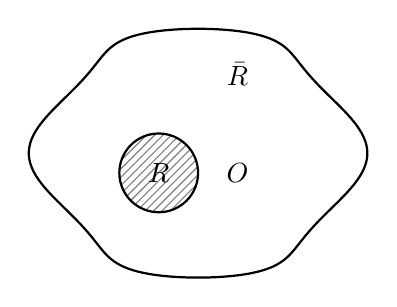
\begin{tikzpicture}
            \draw[thick]
                plot [domain=0:360, samples=200, smooth, variable=\t]
                    (
                        {0.5 + 2*cos(\t) + 0.15*cos(5*\t)},
                        {0.25 + 1.5*sin(\t) + 0.08*sin(1*\t)}
                    )
                    -- cycle;
            \fill[pattern=north east lines, pattern color=black!50] (0,0) circle (0.5);
            \draw[thick] (0,0) circle (0.5);
            \node at (0,0) {\(R\)};
            \node at (1,1.25) {\(\bar R\)};
            \node at (1, 0) {\(O\)};
        \end{tikzpicture}
    \end{figure}

    For an excitation \(\ket{\psi(R)}\) to be local in \(R\), we require that 
    \begin{equation*}
        \braket{\psi(R)|O(\bar{R}) | \psi(R)} = \braket{0|O(\bar{R})|0} ~~\forall~O \text{ in region spacelike to }R
    \end{equation*} 
    That is, the expectation values of operators in regions spacelike separated from \(R\) should be the same as their vacuum expectation values.  \\

    How can we create such a state?\\
    Our first guess would be 
    \begin{equation*}
        \ket{\psi(R)} = \int_R d^4x f(x) \phi(x) \ket{0} 
    \end{equation*}
    We can check if this is indeed a localised expectation, 
    \begin{equation*}
        \braket{\psi(R)|O(\bar{R})|\psi(R)} = \int f(x) f(y) \braket{0|\phi(x) O \phi(y) | 0}
    \end{equation*}
    since \(\phi\) in \(R\) and \(O\) in \(\bar{R}\) must commute, the above should be equal to 
    \begin{equation*}
        \braket{\psi(R)|O(\bar{R})|\psi(R)} = \int f(x) f(y) \braket{0|O\phi(x)  \phi(y) | 0}
    \end{equation*}
    which is not equal to the vacuum expectation value of \(O\). See that even \(\phi(z)\) does not produce a local excitation \textbf{at \(z\)}, since \(\phi(z)\) is obtained by simply setting \(f(x) = \delta(x-z), ~f(y) = \delta(z-y)\) in the above integral.  \\

    What do we need to create a localized excitation?\\
    In order for \(\ket{\psi(R)} = U(R)\ket{0}\) to be a localised excitation, we need 
    \begin{equation*}
        \braket{\psi(R)|O(\bar{R})|\psi(R)} = \braket{0|U^\dagger(R)O(\bar{R})U(R)|0} = \braket{0|O(\bar{R})U^\dagger(R)U(R)|0} = \braket{0|O(\bar{R})|0}
    \end{equation*}
    What this implies is that the operator \(U\) should satisfy \(U^\dagger U = I\), i.e.\ it should be unitary. Therefore 
    \begin{equation*}
        U(R) = \e^{i\int_R f(x)\phi(x) dx}\ket{0}
    \end{equation*}
    is a localised excitation in \(R\). There is no unique localised excitation, there can be many unitary operators in \(R\) that can produce localised excitations. One can also see that since \(\phi\) are Hermitian, the only way to create unitary operators is by exponentiating the \(\phi\)s with a factor of \(i\). If you produce an excitation in a region of space \(\textbf{R}\), it propagates outwards at the speed of light, such that all the region which is timelike to \(\textbf{R}\) is affected, while regions spacelike to \(\textbf{R}\) are not at all affected. \\
    
    Now these localised excitations can never be single particle states. Since the exponential can be written as 
    \begin{equation*}
        \e^{i\int_R f(x)\phi(x) dx}\ket{0} = \left(1 + i\int_R f(x)\phi(x) dx + \frac{1}{2}i\iint_R f(x)f(y)\phi(x)\phi(y) dxdy + \cdots \right)\ket{0}
    \end{equation*}
    the localised excitation is always a superposition of states of all possible particle numbers. 

    \newpage
    \section{Interlude — Symmetries}

    What we mean when we say that the action has symmetry is that when we make a change in the fields \(\phi_i(x) \to \phi_i(x) + \lambda D\phi_i(x)\), (where \(D\phi_i\) is just a notation and can denote any function, but is usually a function of original \(\phi_i\)s and \(\lambda\) is a parameter to keep track of order of terms), the action remains invariant. \\
    For this to be true, the Lagrangian density should transform as 
    \begin{equation*}
        \ld \to \ld + \del_\mu K^\mu
    \end{equation*}
    Now this invariance should hold for all the field configurations, and not just some special ones, i.e.\ the configurations which satisfy the equations of motion. For the configurations which satisfy the equations of motion, the requirement is identically satisfied, since we define the equations of motion as those configurations for which the small variations of fields do not change the action.\\ 

    \subsection{Noether's Theorem}
    When \(\ld\) has a symmetry, there is a conserved current of the form
    \begin{equation*}
        \del_\mu j^\mu = 0
    \end{equation*} 
    \textit{only for the solutions of the equations of motion}.\\

    Proof —\\
    Under the above transformation,
    \begin{align*}
        &\delta \ld = \left( \frac{\delta \ld}{\delta \phi_i} D\phi_i  + \frac{\delta \ld}{\delta \del_\mu \phi_i} \del_\mu D\phi_i \right) = \del_\mu K^\mu \\
        \implies & \left( \frac{\delta \ld}{\delta \phi_i} D\phi_i  -\del_\mu \frac{\delta \ld}{\delta \del_\mu \phi_i} D\phi_i + \del_\mu \left( \frac{\delta \ld}{\delta \del_\mu \phi_i} D\phi_i \right)  \right) = \del_\mu K^\mu 
    \end{align*}
    When we are on-shell (i.e. when \(\phi\) satisfies the equation of motion), the first two term sum to 0, and we are left with 
    \begin{equation*}
        \del_\mu \left( \frac{\delta \ld}{\delta \del_\mu \phi_i} D\phi_i \right) = \del_\mu K^\mu
    \end{equation*}
    which implies that  
    \begin{equation*}
        \del_\mu j^\mu(x) =0, ~\text{ where  } j^\mu = \frac{\delta \ld}{\delta \del_\mu \phi_i} D\phi_i  - K^\mu 
    \end{equation*}

    Noether's current is not something new, it is just re-expressing the equations of motion. Noether's current has inherent ambiguity in definition, because we can always add a divergence free \(4-\)vector to it, i.e.\ we can add terms of the form \(\epsilon^{\mu\nu} \del_\nu \phi\) where \(\epsilon\) is antisymmetric tensor, since \(\del_\mu \epsilon^{\mu\nu} \del_\nu \phi = 0\). But nevertheless this is a powerful statement and allows us to derive conclusions without having to do tedious calculations.\\

    When we have a conserved current, we have a conserved charge.
    \begin{equation*}
        \del_0 \int j^0 d^3\textbf{x} + \int d^3\textbf{x} \del_i j^i = 0 \implies \del_t \int j^0 d^3\textbf{x} = 0
    \end{equation*}
    since the second term is a total divergence. What this tells is that the quantity 
    \begin{equation*}
        Q = \int j^0 d^3\textbf{x}
    \end{equation*} 
    is conserved. All conservation of laws that we have known so far arise in this very fashion, and are consequences of the Noether's theorem.\\

    There is another derivation of the Noether's theorem, which is at the level of action. Suppose we have a symmetry under 
    \begin{equation*}
        \phi \to \phi + \lambda D\phi
    \end{equation*}
    which does not change \(S\).\\
    Now imagine a spacetime dependent variation, 
    \begin{equation*}
        \phi \to \phi + \lambda(x) D\phi
    \end{equation*}
    The action is not invarient under this transformation. The Lagrangian, upto first order in \(\lambda\) changes as 
    \begin{equation*}
        \ld \to \ld + \lambda(x) \del_\mu(K^\mu) + \del_\mu(\lambda(x)) P^\mu
    \end{equation*}
    since these are the only terms that are Lorentz invariant and first order in \(\lambda\).\\
    The action transforms as 
    \begin{align*}
        S \to &S + \int d^4x~ \lambda(x) \del_\mu(K^\mu) + \del_\mu(\lambda(x)) P^\mu\\
        = & S + \int d^4x ~ \lambda(x) \del_\mu (K^\mu - P^\mu)
    \end{align*}
    On solutions to equations of motions, the action should be invariant under these transformations too. Therefore 
    \begin{equation*}
        \del_\mu (K^\mu - P^\mu) = 0
    \end{equation*}
    Now what is \(P^\mu\)? \\
    Under the given transformation, the Lagrangian changes as 
    \begin{equation*}
        \ld \to \ld + \left( \frac{\delta \ld}{\delta \phi}\lambda(X) D\phi +  \frac{\delta \ld}{\delta \del_\mu \phi} \del_\mu(\lambda(x) D\phi) \right)
    \end{equation*}
    from which we can see that \(P^\mu\) is simply the part that multiplies to \(\del_\mu \lambda(x)\), which is 
    \begin{equation*}
        P^\mu = \frac{\delta \ld}{\delta \del_\mu \phi} D\phi
    \end{equation*}

    \subsection{Applications}
    Let us look at some applications of the Noether's theorem
    \subsubsection{Spacetime translations}
    Consider \(x^\mu \to x^\mu + a^\mu\).\\
    When \(\ld\) doesn't explicitly depend on position, this is a symmetry. In the language of fields, this transformation is 
    \begin{equation*}
        \phi \to \phi + \lambda \del_\mu \phi^\mu 
    \end{equation*}
    where \(\lambda\) is just to keep track of orders.\\

    Since \(\ld\) is a Lorentz scalar, 
    \begin{equation*}
        \ld \to \ld + \lambda a^\mu \del_\mu \ld \implies K^\mu =  a^\mu \ld
    \end{equation*}

    Therefore, the conserved current is 
    \begin{equation*}
        j^\mu = \frac{\delta \ld}{\delta \del_\mu \phi}a^\nu  \del_\nu \phi  - a^\nu \delta_\nu^\mu \ld
    \end{equation*}
    Now this current is conserved for all possible \(a^\mu\) which means that 
    \begin{equation*}
        T_\nu^\mu = \frac{\delta \ld}{\delta \del_\mu \phi} \del_\nu \phi  -  \delta_\nu^\mu \ld \implies T^{\mu\nu} = \frac{\delta \ld}{\delta \del_\mu \phi} \del^\nu \phi  -  \eta^{\mu\nu} \ld
    \end{equation*}
    must be conserved. This is called stress-energy tensor and this is conserved. Let us check what this is for few cases 
    \begin{equation*}
        T^{00} = \frac{\delta \ld}{\delta \dot{\phi}}  \dot{\phi} - \ld = \mathcal{H}
    \end{equation*}
    which is the Hamiltonian density. Integrating this over all space gives the Hamiltonian which is the energy, and this shows that energy is conserved.
    \begin{equation*}
        T^{0i} = \frac{\delta \ld}{\delta \dot{\phi}} \del^i \phi
    \end{equation*}
    the corresponding conserved charge is 
    \begin{equation*}
        P^i =  \int d^3\textbf{x} \frac{\delta \ld}{\delta \dot{\phi}} \del^i \phi
    \end{equation*}
    which is nothing but the spatial momentum in \(i\)th direction as we had defined previously. The stress tensor therefore gives \(4\) conserved charges (we need to keep \(\mu = 0\) and integrate, and there are \(4\) choice of \(\nu\)) which are energy and the three components of momentum.\\ 

    The formula for stress-tensor is not manifestly symmetric in \(\mu\) and \(\nu\), but we can use the ambiguity that we discussed to subtract the antisymmetric part and make it symmetric. But in most cases of physical interest, stress-tensor is explicitly symmetric.

    \subsubsection{Lorentz transformation}
    Lorentz transformation 
    \begin{equation*}
        \tilde{x}^\mu = \Lambda\indices{^\mu_\nu} x^\nu
    \end{equation*}
    The requirement is that the transformation preserves vector inner products 
    \begin{equation*}
        \tilde{x}^\mu\tilde{y}^\nu \eta_{\mu\nu} = x^\mu y^\nu \eta_{\mu\nu} \implies \Lambda\indices{^\rho_\mu} \Lambda\indices{^\sigma_\nu} \eta_{\rho\sigma} =\eta_{\mu\nu} 
    \end{equation*}

    An infinitesimal transformation of \(x\) would be 
    \begin{equation*}
        x^\mu \to x^\mu + \lambda \epsilon\indices{^\mu_\nu} x^\nu
    \end{equation*}
    For this to be a Lorentz transformation 
    \begin{align*}
        &(x^\mu + \lambda \epsilon\indices{^\mu_\nu} x^\nu)(y_\mu + \lambda \epsilon\indices{_\mu_\nu} y^\nu) = x^\mu y_\mu \\
        \implies & x^\mu y_\mu + \lambda \epsilon\indices{^\mu_\nu} x^\nu y_\mu + \lambda\epsilon_{\mu\nu}x^\mu y^\nu + O(\lambda^2) = x^\mu y_\mu\\
        \implies & \epsilon_{\mu\nu}x^\nu y^\mu + \epsilon_{\mu\nu} x^\mu y^\nu = 0
    \end{align*}
    Now since in the first term, \(\mu\) and \(\nu\) are dummy indices, we can interchange them to get 
    \begin{equation*}
        \left(\epsilon_{\nu\mu}+ \epsilon_{\mu\nu}\right) x^\mu y^\nu = 0\implies  \epsilon_{\nu\mu}= - \epsilon_{\mu\nu}
    \end{equation*}
    Which implies that the \(\epsilon_{\mu\nu}\) is an antisymmetric tensor. (Notice that this would not work if we compare tensors with one upper and one upper index). There are 6 components to the antisymmetric tensor, and therefore 6 conserved currents — three for boosts and three for rotations. As an example consider \(\epsilon_{01} = 1,~\epsilon_{10} = -1\) rest all 0. Under this 
    \begin{equation*}
        \delta x^0 = \lambda x^1,~~\delta x^1 = \lambda x^0
    \end{equation*}
    which are infinitesimal boosts. If \(\epsilon_{12} = 1,~\epsilon_{21} = -1\), then 
    \begin{equation*}
        \delta x^1 = -\lambda x^2,~~\delta x^2 = \lambda x^1
    \end{equation*}
    This is an infinitesimal rotation. \\

    Under Lorentz transformation, the fields transform as 
    \begin{equation*}
        \delta x^\mu = \lambda \epsilon\indices{^\mu_\nu} x^\nu \implies \delta \phi =\lambda \del_\mu \phi \epsilon\indices{^\mu_\nu} x^\nu
    \end{equation*}

    Under this kind of transformation, the lagrangian density also transforms as 
    \begin{equation*}
        \delta \ld = \lambda (\del_\mu \ld) \epsilon\indices{^\mu_\nu} x^\nu 
    \end{equation*}
    Now since \(\del_\mu (\epsilon\indices{^\mu_\nu} x^\nu) = \delta\indices{^\nu_\mu}\epsilon\indices{^\mu_\nu} = \eta^{\mu\nu}\epsilon_{\mu\nu} = 0\) (\(\because\) \(eta\) is symmetric and \(\epsilon\) is antisymmetric) \textcolor{red}{(another way to look at this is that \(\delta\indices{^\nu_\mu}\epsilon\indices{^\mu_\nu} = \mathrm{Tr}\epsilon = 0\))} we can add this term to make the change in lagrangian density a total derivative 
    \begin{equation*}
        \delta ld = \lambda \del_\mu (\ld \epsilon\indices{^\mu_\nu} x^\nu)
    \end{equation*}
    To proceed, let us consider an explicit example of a theory, the lagrangian density we have already considered. For this theory, 
    \begin{equation*}
        \frac{\delta \ld}{\delta \del_\mu \phi} = \del^\mu \phi
    \end{equation*}
    and therefore, 
    \begin{equation*}
        j^\mu = \del^\mu \phi \del_\rho \phi \epsilon\indices{^\rho_\nu}x^\nu - \ld \epsilon\indices{^\mu_\nu} x^\nu
    \end{equation*}
    Since this should be conserved for all \(\epsilon\), we need to pull it out of the equation as 
    \begin{equation*}
        j^\mu = (\del^\mu \phi \del^\rho \phi x^\nu - \ld \eta\indices{^\rho^\mu} x^\nu)\epsilon\indices{_\rho_\nu}
    \end{equation*}
    The conserved current is therefore the antisymmetric part of 
    \begin{equation*}
        \del^\mu \phi \del^\rho \phi x^\nu - \ld \eta\indices{^\rho^\mu} x^\nu
    \end{equation*}
    since the derivative of the symmetric part is identically zero, owing to the presence of \(\epsilon\). Therefore the conserved current is 
    \begin{equation*}
        M^{\mu\nu\rho} = (\del^\mu \phi \del^\rho \phi x^\nu - \ld \eta\indices{^\rho^\mu} x^\nu) - (\rho\leftrightarrow \nu)
    \end{equation*}
    There are 6 possible choices of \(\rho\) and \(\nu\) for the antisymmetric part, and therefore 6 conserved currents. \\

    The above quantity is exactly equal to 
    \begin{equation*}
        M^{\mu\nu\rho} = x^\nu T^{\mu\rho} - x^\rho T^{\mu\nu}
    \end{equation*}
    where \(T\) is the stress tensor. The six conserved charges are 
    \begin{equation*}
        Q^{\nu\rho} = \int  x^\nu T^{0\rho} - x^\rho T^{0\nu} d^3\textbf{x}
    \end{equation*}

    The different cases —\\
    \begin{equation*}
        Q^{ij} = \int  x^i T^{0j} - x^j T^{0i} d^3\textbf{x}
    \end{equation*}
    This is angular momentum associated with the plane of rotation \(ij\).
    \begin{equation*}
        Q^{0i} = \int  x^0 T^{0i} - x^i T^{00} d^3\textbf{x}
    \end{equation*}
    Let us write it in a slightly different way. \(\int T^{01} d^3\textbf{x} = P^i\), meaning 
    \begin{equation*}
        Q^{0i} = tP^i - \int x^i T^{00} d^\textbf{x}
    \end{equation*}
    Differentiating with respect to time (and using momentum is conserved),
    \begin{equation*}
        P^i - \frac{d}{dt} \int x^i T^{tt} d^3\textbf{x} = 0 \implies P^i - \left(\int  T^{tt}d^3\textbf{x} \right)\times \frac{d}{dt} \frac{\int x^i T^{tt} d^3\textbf{x}}{\int  T^{tt} d^3\textbf{x}}
    \end{equation*}
    Since \(T^{tt}\) is simply the mass density, the integral in the brackets is simply the total mass, and the object getting differentiated is the position of the center of mass. That is 
    \begin{equation*}
        P^i = M\frac{d}{dt} x^i_{COM}
    \end{equation*}
    which is just the classical defninition of momentum. 

    \subsubsection{Internal Symmetries}
    So far we discussed transformations in \(\phi\) due to changes to spacetime. Now we will discuss something different. Consider a theory with two fields, 
    \begin{equation*}
        \ld = \frac{1}{2} (\del_\mu \phi_1)^2 + \frac{1}{2} (\del_\mu \phi_1)^2 - \frac{m^2}{2} \phi_1^2-\frac{m^2}{2} \phi_2^2
    \end{equation*} 
    This theory has a continous symmetry under rotations of \(\phi_1\) into \(\phi_2\), i.e. 
    \begin{equation*}
        \phi_1 \to \cos\theta \phi_1 - \sin\theta \phi_2,~~ \phi_2\to \cos\theta \phi_2 + \sin\theta \phi_1
    \end{equation*}
    This transformation leaves the lagrangian density unchanged. \\
    infinitesimally, the above transformation looks like 
    \begin{equation*}
        \delta \phi_1 = - \phi_2,~~\delta \phi_2 = \phi_1
    \end{equation*}
    The associated current is 
    \begin{equation*}
        j^\mu =  \phi_1 \del^\mu \phi_2 - \phi_2 \del^\mu \phi_1
    \end{equation*}
    The associated charge is 
    \begin{equation*}
        Q = \int \phi_1 \del^0 \phi_2 - \phi_2 \del^0 \phi_1 d^3\textbf{x}
    \end{equation*}
    Charges like electric charge etc.\ are of this form. \\

    These fields are real fields. However we can combine these two into one complex object as
    \begin{equation*}
        \chi = (\phi_1 + i\phi_2)\frac{1}{\sqrt{2}},~~\chi^* = (\phi_1 - i\phi_2)\frac{1}{\sqrt{2}}
    \end{equation*}
    With this, 
    \begin{equation*}
        \frac{1}{2}(\phi_1^2 + \phi_2^2) = |\chi|^2
    \end{equation*}
    and 
    \begin{equation*}
        \frac{1}{2} ((\del_\mu \phi_1)^2 + (\del_\mu \phi_2)^2) = |\del_\mu \chi|^2
    \end{equation*}
    Therefore, the Lagrangian density becomes
    \begin{equation*}
        \ld = |\del_\mu \chi|^2 - m^2 |\chi|^2
    \end{equation*}
    In this language, the symmetry is
    \begin{equation*}
        \chi \to \e^{i\alpha} \chi,~~\chi^* \to \e^{-i\alpha}\chi^*
    \end{equation*}
    The corresponding current is 
    \begin{equation*}
        j^\mu = i((\del_\mu \chi^*) \chi - (\del_\mu\chi)\chi^*)
    \end{equation*}
    Since \(phi_1\) and \(\phi_2\) transformed into each other, they are not the fields corresponding to particles of positive and negative charges.\ \(\chi\) and \(\chi^*\) are the fields that correspond to particles of positive and negative charges. This is an example of \(U(1)\) internal symmetry. We can have theories with more elaborate symmetries like \(SU(N), Sp(N)\) etc.

    \newpage 
    \section{The Interaction Picture}
    So far, we discussed free field theories, and we want to extend our discussions interacting theories. Before that, let us discuss what kind of questions can we ask in the presence of interactions. \\

    The most general kind of question would be 
    \begin{figure}[h]
        \centering
        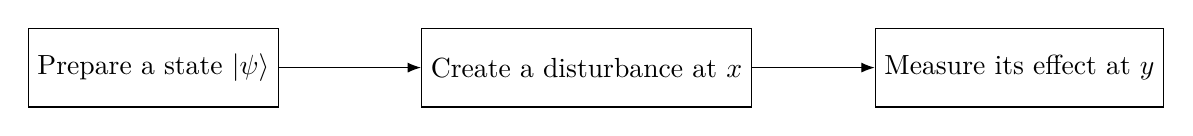
\begin{tikzpicture}[>=Latex,node distance=5.5cm]
            \node[draw, rectangle, minimum width=3cm, minimum height=1cm] (A) {Prepare a state \(\ket{\psi}\)};
            \node[draw, rectangle, right of=A, minimum width=3cm, minimum height=1cm] (B) {Create a disturbance at \(x\)};
            \node[draw, rectangle, right of=B, minimum width=3cm, minimum height=1cm] (C) {Measure its effect at \(y\)};

            % Draw the arrows
            \draw[->] (A) -- (B);
            \draw[->] (B) -- (C);

        \end{tikzpicture}
    \end{figure}

    However, it turns out that in QFT, although we can ask these questions, a lot of focus is on slightly \textit{simpler} questions.\\
    The simpler question is 
    \begin{figure}[h]
        \centering
        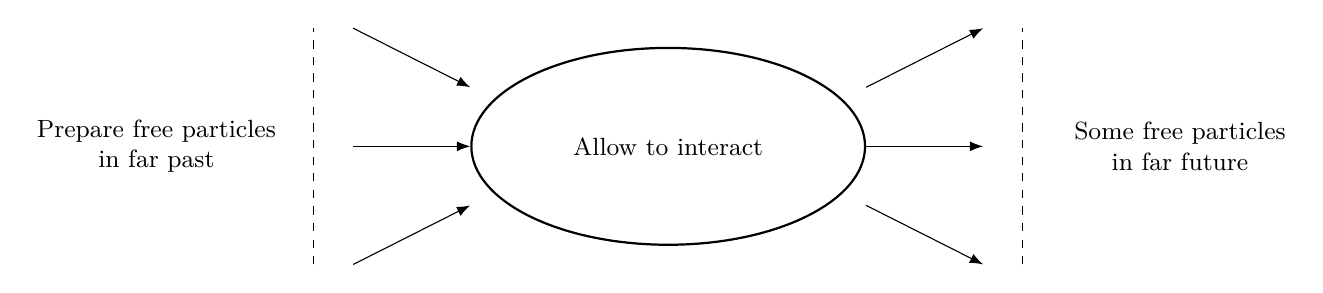
\begin{tikzpicture}[>=Latex, every node/.style={font=\small, align=center}]

            % Left and right text
            \node (in) at (-6.5,0) {Prepare free particles\\in far past};
            \node (out) at ( 6.5,0) {Some free particles \\in far future};

            \draw[dashed] (-4.5, -1.5) -- (-4.5, 1.5);
            \draw[dashed] (4.5, -1.5) -- (4.5, 1.5);

            \node[ellipse, draw, thick,
                minimum width=5cm, minimum height=2.5cm] (proc) 
            at (0,0) {Allow to interact};

            % Converging arrows (left → centre)
            %   start at (-6, +2),(-6,0),(-6,-2)
            %   end at proc.west + (0,+1),(0,0),(0,-1)
            \foreach \sy/\ey in {1.5/0.75, 0/0, -1.5/-0.75} {
                \draw[->] (-4,\sy) -- ($(proc.west)+(0,\ey)$);
            }

            % Diverging arrows (centre → right)
            %   start at proc.east + (0,+1),(0,0),(0,-1)
            %   end at (6,+2),(6,0),(6,-2)
            \foreach \ey/\sy in {0.75/1.5, 0/0, -0.75/-1.5} {
                \draw[->] ($(proc.east)+(0,\ey)$) -- (4,\sy);
            }

        \end{tikzpicture}
    \end{figure}

    That is, we create free particles in far past, let them evolve and interect, and ask what are the free particles and their properties in far future. This kind of question is answered by something called the \(S\) matrix. One might think that this is less general than the other question, but in fact it turns out that it has all the information we want to have about the theory. \\

    Why we talk about \(S\) matrix?
    \begin{enumerate}
        \item Experiments — most physics we learn from experiments is from this kind of experiments. 
        \item Theoretical reasons — two theoretical reasons \begin{itemize}
            \item \(S\) matrix is an unambigously decided observable. That is if we ask the question like what is the correlator 
            \begin{equation*}
                \braket{\psi | \phi(x_1) \cdots \phi(x_n)| \psi}
            \end{equation*}
            this is very ambigous. This is because in interacting theory, there is no unambigous \textit{definition} of field. One can always redefine the fields at the cost of adding interaction terms, without altering the physical content of the theory. When the fields are free and don't interact, there is 'a' free field, and field redefinitions do not obey the equations of motions whereas the original field obeys. But in case of interacting theories, no fields obey the equation of motion, and therefore there is no more unique field.\\
            There is a class of field theories called conformal field theories, where there are other principles that allows one to uniquely identify field variables even in the case of interactions, and there we can talk about the first type of questions. But in general \(S\) matrix is unambigously defined since all we talk about is free theories in far past and future.
            \item In Quantum Gravity, maybe only the \(S\) matrix makes sense. The reason for that is that the first type of questions involve some local questions about what happens in some local regions of spacetime, and when the metric itself is fluctuating and spacetime itself is fluctuating, such questions are not well defined. But when we ask the second type of questions, in far past and future, where such fluctuations are not present, it is perfectly well defined. 
        \end{itemize}
    \end{enumerate}

    Therefore there are good reasons to consider the \(S\) matrix. Now we develop the machinery needed to calculate these \(S\) matrices.




\end{document}
